%%%%%%%%%%%%%%%%%%%%%%%%%%%%%%%%%%%%%%%%%%%%%%%%%%%%%%%%%%%%%%%%%%%%%%
%%  Copyright by Wenliang Du.                                       %%
%%  This work is licensed under the Creative Commons                %%
%%  Attribution-NonCommercial-ShareAlike 4.0 International License. %%
%%  To view a copy of this license, visit                           %%
%%  http://creativecommons.org/licenses/by-nc-sa/4.0/.              %%
%%%%%%%%%%%%%%%%%%%%%%%%%%%%%%%%%%%%%%%%%%%%%%%%%%%%%%%%%%%%%%%%%%%%%%

\documentclass[11pt]{article}

\usepackage[most]{tcolorbox}
\usepackage{times}
\usepackage{epsf}
\usepackage{epsfig}
\usepackage{amsmath, alltt, amssymb, xspace}
\usepackage{wrapfig}
\usepackage{fancyhdr}
\usepackage{url}
\usepackage{verbatim}
\usepackage{fancyvrb}
\usepackage{adjustbox}
\usepackage{listings}
\usepackage{color}
\usepackage{subfigure}
\usepackage{cite}
\usepackage{sidecap}
\usepackage{pifont}
\usepackage{mdframed}
\usepackage{textcomp}
\usepackage{enumitem}


% Horizontal alignment
\topmargin      -0.50in  % distance to headers
\oddsidemargin  0.0in
\evensidemargin 0.0in
\textwidth      6.5in
\textheight     8.9in 

\newcommand{\todo}[1]{
\vspace{0.1in}
\fbox{\parbox{6in}{TODO: #1}}
\vspace{0.1in}
}


\newcommand{\unix}{{\tt Unix}\xspace}
\newcommand{\linux}{{\tt Linux}\xspace}
\newcommand{\minix}{{\tt Minix}\xspace}
\newcommand{\ubuntu}{{\tt Ubuntu}\xspace}
\newcommand{\setuid}{{\tt Set-UID}\xspace}
\newcommand{\openssl} {\texttt{openssl}}


\pagestyle{fancy}
\lhead{\bfseries SEED Labs}
\chead{}
\rhead{\small \thepage}
\lfoot{}
\cfoot{}
\rfoot{}


\definecolor{dkgreen}{rgb}{0,0.6,0}
\definecolor{gray}{rgb}{0.5,0.5,0.5}
\definecolor{mauve}{rgb}{0.58,0,0.82}
\definecolor{lightgray}{gray}{0.90}


\lstset{%
  frame=none,
  language=,
  backgroundcolor=\color{lightgray},
  aboveskip=3mm,
  belowskip=3mm,
  showstringspaces=false,
%  columns=flexible,
  basicstyle={\small\ttfamily},
  numbers=none,
  numberstyle=\tiny\color{gray},
  keywordstyle=\color{blue},
  commentstyle=\color{dkgreen},
  stringstyle=\color{mauve},
  breaklines=true,
  breakatwhitespace=true,
  tabsize=3,
  columns=fullflexible,
  keepspaces=true,
  escapeinside={(*@}{@*)}
}

\newcommand{\newnote}[1]{
\vspace{0.1in}
\noindent
\fbox{\parbox{1.0\textwidth}{\textbf{Note:} #1}}
%\vspace{0.1in}
}


%% Submission
\newcommand{\seedsubmission}{You need to submit a detailed lab report, with screenshots,
to describe what you have done and what you have observed.
You also need to provide explanation
to the observations that are interesting or surprising.
Please also list the important code snippets followed by
explanation. Simply attaching code without any explanation will not
receive credits.}

%% Book
\newcommand{\seedbook}{\textit{Computer \& Internet Security: A Hands-on Approach}, 2nd
Edition, by Wenliang Du. See details at \url{https://www.handsonsecurity.net}.}

%% Videos
\newcommand{\seedisvideo}{\textit{Internet Security: A Hands-on Approach},
by Wenliang Du. See details at \url{https://www.handsonsecurity.net/video.html}.}

\newcommand{\seedcsvideo}{\textit{Computer Security: A Hands-on Approach},
by Wenliang Du. See details at \url{https://www.handsonsecurity.net/video.html}.}

%% Lab Environment
\newcommand{\seedenvironment}{This lab has been tested on our pre-built
Ubuntu 16.04 VM, which can be downloaded from the SEED website. }

\newcommand{\seedenvironmentA}{This lab has been tested on our pre-built
Ubuntu 16.04 VM, which can be downloaded from the SEED website. }

\newcommand{\seedenvironmentB}{This lab has been tested on our pre-built
Ubuntu 20.04 VM, which can be downloaded from the SEED website. }

\newcommand{\seedenvironmentAB}{This lab has been tested on our pre-built
Ubuntu 16.04 and 20.04 VMs, which can be downloaded from the SEED website. }

\newcommand{\nodependency}{Since we use containers to set up the lab environment, 
this lab does not depend too much on our SEED VM. You can do this lab
using other VMs or physical machines. }







\newcommand{\seedlabcopyright}[1]{
\vspace{0.1in}
\fbox{\parbox{6in}{\small Copyright \copyright\ {#1}\ \ by Wenliang Du.\\
      This work is licensed under a Creative Commons
      Attribution-NonCommercial-ShareAlike 4.0 International License.
      If you remix, transform, or build upon the material, 
      this copyright notice must be left intact, or reproduced in a way that is reasonable to
      the medium in which the work is being re-published.}}
\vspace{0.1in}
}






\newcommand{\pkiFigs}{./Figs}

\newcommand{\OpenSSL} {\texttt{OpenSSL}\xspace}
\newcommand{\pkiserver}{\texttt{SEEDPKILab2020.com}\xspace} 

\lhead{\bfseries SEED Labs -- PKI Lab}


\begin{document}

\begin{center}
{\LARGE Public-Key Infrastructure (PKI) Lab}
\end{center}

\seedlabcopyright{2018}



% *******************************************
% SECTION
% ******************************************* 
\section{Overview}



Public key cryptography is the foundation of today's secure
communication, but it is subject
to man-in-the-middle attacks when one side of communication sends its
public key to the other side.  The fundamental problem is
that there is no easy way to verify the ownership of a public key, i.e., given a public key and
its claimed owner information, how do we ensure that the public key is indeed owned by
the claimed owner? The Public Key Infrastructure~(PKI) is a practical solution
to this problem.


The learning objective of this lab is for students to gain the first-hand 
experience on PKI. SEED labs have a series of labs focusing on the public-key cryptography, and 
this one focuses on PKI. By doing the tasks in this lab, students should be able to gain a 
better understanding of how PKI works, how PKI is used to protect the Web, and
how Man-in-the-middle attacks can be defeated by PKI. Moreover, students will be able to
understand the root of the trust in the public-key infrastructure, and what problems 
will arise if the root trust is broken.  This lab covers the following topics:

\begin{itemize}[noitemsep]
\item Public-key encryption
\item Public-Key Infrastructure (PKI)
\item Certificate Authority (CA) and root CA 
\item X.509 certificate and self-signed certificate
\item Apache, HTTP, and HTTPS
\item Man-in-the-middle attacks
\end{itemize}



\paragraph{Readings.}
Detailed coverage of PKI can be found in the following:

\begin{itemize}
\item Chapter 23 of the SEED Book, \seedbook
\end{itemize}


\paragraph{Related labs.}
A topic related to this lab is the Transport Layer Security (TLS), which is based on  
PKI. We have a separate lab for TLS.
In addition, we have a lab called \textit{RSA Public-Key Encryption and Signature Lab}, 
which focuses on the algorithm part of the public-key cryptography.


\paragraph{Lab environment.} \seedenvironment 



% *******************************************
% SECTION
% ******************************************* 
\section{Lab Tasks}


% -------------------------------------------
% SUBSECTION
% ------------------------------------------- 
\subsection{Task 1: Becoming a Certificate Authority (CA)}

A Certificate Authority (CA) is a trusted entity that issues digital certificates. 
The digital certificate certifies the ownership of a public key by 
the named subject of the certificate. A number of commercial 
CAs are treated as root CAs; VeriSign is the largest CA at the time of 
writing. Users who want to get digital certificates issued
by the commercial CAs need to pay those CAs.


In this lab, we need to create digital certificates, but we are not going to pay
any commercial CA. We will become a root CA ourselves, and then use this CA to 
issue certificate for others (e.g. servers). In this task, we will make
ourselves a root CA, and generate a certificate for this CA. Unlike 
other certificates, which are usually signed by another CA, the root CA's 
certificates are self-signed. Root CA's certificates are usually pre-loaded
into most operating systems, web browsers, and other software that rely on PKI.
Root CA's certificates are unconditionally trusted.


\paragraph{The Configuration File {\tt openssl.conf}.}
In order to use \OpenSSL to create certificates, you have to have a 
configuration file.
The configuration file usually has an extension
{\tt .cnf}. It is used by three \OpenSSL commands: {\tt ca}, {\tt req} and {\tt x509}. 
The manual page of \texttt{openssl.conf} can be found using Google search.
You can also get a  copy of the configuration file from \path{/usr/lib/ssl/openssl.cnf}. 
After copying this file into your current directory, you need to 
create several sub-directories as specified in the configuration file (look
at the {\tt [CA\_default]} section):


\begin{lstlisting}
   dir             = ./demoCA        # Where everything is kept
   certs           = $dir/certs      # Where the issued certs are kept
   crl_dir         = $dir/crl        # Where the issued crl are kept
   new_certs_dir   = $dir/newcerts   # default place for new certs.
   database        = $dir/index.txt  # database index file.
   serial          = $dir/serial     # The current serial number
\end{lstlisting}

For the \texttt{index.txt} file, simply create an empty file. For 
the \texttt{serial} file, put a single number in string format (e.g. 1000) in the file.
Once you have set up the configuration file \texttt{openssl.cnf}, 
you can create and issue certificates.


\paragraph{Certificate Authority (CA).} 
As we described before, we need to generate a self-signed certificate for our
CA. This means that this CA is totally trusted, and its certificate will serve
as the root certificate.  You can run the following command to generate  
the self-signed certificate for the CA:


\begin{lstlisting}[backgroundcolor=]
$ openssl req -new -x509 -keyout ca.key -out ca.crt -config openssl.cnf
\end{lstlisting}

You will be prompted for information and a password. Do not lose this password,
because you will have to type the passphrase 
each time you want to use this CA to sign certificates for others.
You will also be asked to fill in some information,
such as the Country Name, Common Name, etc. 
The output of the command are stored in two files: {\tt ca.key} and 
{\tt ca.crt}. The file {\tt ca.key} contains the 
CA's private key, while {\tt ca.crt} contains the public-key certificate.



% -------------------------------------------
% SUBSECTION
% ------------------------------------------- 
\subsection{Task 2: Creating a Certificate for \pkiserver}

Now, we become a root CA, we are ready to sign digital certificates for 
our customers. Our first customer is a company called \pkiserver.
For this company to get a digital certificate from a CA, it needs to
go through three steps.


\paragraph{Step 1: Generate public/private key pair.}
The company needs to first create its own public/private key pair. We can run  
the following command to generate an RSA key pair (both private and public keys).  
You will also be required to provide a password to encrypt the private 
key (using the AES-128 encryption algorithm, as is specified in the command option). 
The keys will be stored in the file \texttt{server.key}:

\begin{lstlisting}[backgroundcolor=]
$ openssl genrsa -aes128 -out server.key 1024
\end{lstlisting}

The \texttt{server.key} is an encoded text file (also encrypted), 
so you will not be able to see the actual content, such as the modulus, private exponents, etc. To see
those, you can run the following command:

\begin{lstlisting}[backgroundcolor=]
$ openssl rsa -in server.key -text
\end{lstlisting}



\paragraph{Step 2: Generate a Certificate Signing Request (CSR).}
Once the company has the key file, it should generates a Certificate Signing Request (CSR), 
which basically includes the company's public key. 
The CSR will be sent to the CA, who will generate a certificate 
for the key (usually after ensuring that identity information in 
the CSR matches with the server's true identity). Please 
use \pkiserver as the common name of the certificate 
request.

\begin{lstlisting}[backgroundcolor=]
$ openssl req -new -key server.key -out server.csr -config openssl.cnf
\end{lstlisting}


It should be noted that the above command is quite similar to the one
we used in creating the self-signed certificate for the CA. The only
difference is the {\tt -x509} option. Without it, the command 
generates a request; with it, the command generates a self-signed 
certificate.


\paragraph{Step 3: Generating Certificates.}
The CSR file needs to have the CA's signature to form a certificate. In 
the real world, the CSR files are usually sent to a trusted CA for their 
signature. In this lab, we will use our own trusted CA 
to generate certificates. The following command turns the 
certificate signing request~({\tt server.csr}) into 
an X509 certificate~({\tt server.crt}), using the CA's
{\tt ca.crt} and {\tt ca.key}:

\begin{lstlisting}[backgroundcolor=]
$ openssl ca -in server.csr -out server.crt -cert ca.crt -keyfile ca.key \
             -config openssl.cnf
\end{lstlisting}


If \OpenSSL refuses to generate certificates, it is very likely that
the names in your requests do not match with those of CA. The matching
rules are specified in the configuration file (look at 
the \texttt{[policy\_match]} section). You can change the names of your 
requests to comply with the policy, or you can change the 
policy.  The configuration file 
also includes another policy (called \texttt{policy\_anything}), 
which is less restrictive. You can choose that policy by
changing the following line: 

\begin{lstlisting}[backgroundcolor=]
   "policy = policy_match"  change to "policy = policy_anything".
\end{lstlisting} 



% -------------------------------------------
% SUBSECTION
% ------------------------------------------- 
\subsection{Task 3: Deploying Certificate in an HTTPS Web Server}

In this lab, we will explore how public-key certificates 
are used by websites to secure web browsing. We will set up
an HTTPS website using \openssl's built-in web server. 


\paragraph{Step 1: Configuring DNS.}
We choose \pkiserver as the name of our website.
To get our computers recognize this name,
let us add the following entry to \texttt{/etc/hosts}; this entry
basically maps the hostname \pkiserver to 
our localhost (i.e., 127.0.0.1):

   
\begin{lstlisting}[backgroundcolor=]
   127.0.0.1  SEEDPKILab2018.com
\end{lstlisting}


\paragraph{Step 2: Configuring the web server.}
Let us launch a simple web server with the certificate 
generated in the previous task. \OpenSSL allows us 
to start a simple web server using the \texttt{s\_server} command: 

\begin{lstlisting}
  # Combine the secret key and certificate into one file
  % cp server.key server.pem
  % cat server.crt >> server.pem
 
  # Launch the web server using server.pem
  % openssl s_server -cert server.pem -www
\end{lstlisting}

By default, the server will listen on port {\tt 4433}. You can alter that using 
the {\tt -accept} option. Now, you can access the server using the following
URL: \url{https://SEEDPKILab2018.com:4433/}.
Most likely, you will get an error message from the browser. In Firefox, you will
see a message like the following:
{\em ``seedpkilab2018.com:4433 uses an invalid security certificate.
The certificate is not trusted because the issuer certificate is unknown''.}


\paragraph{Step 3: Getting the browser to accept our CA certificate.}
Had our certificate been assigned by VeriSign, we will not have such an error
message, because VeriSign's certificate is very likely preloaded into
Firefox's certificate repository already. Unfortunately, the 
certificate of \pkiserver is signed by our own CA (i.e., using 
{\tt ca.crt}), and this CA is not recognized by Firefox. There are two ways to
get Firefox to accept our CA's self-signed certificate. 

\begin{itemize}

\item We can request Mozilla to include our CA's certificate in its Firefox software, so
everybody using Firefox can recognize our CA.  This is how the real CAs, such as VeriSign, get
their certificates into Firefox. Unfortunately, our own CA does not have a large enough market
for Mozilla to include our certificate, so we will not pursue this direction.

\item {\bf Load {\tt ca.crt} into Firefox:} We can manually add our CA's certificate to the
Firefox browser by clicking the following menu sequence:

\begin{lstlisting}[backgroundcolor=]
   Edit -> Preference -> Privacy & Security -> View Certificates.
\end{lstlisting}

You will see a list of certificates that are already accepted by Firefox. From here, we 
can ``import'' our own certificate. Please import {\tt ca.crt}, and select the
following option: ``Trust this CA to identify web sites''.  You will see that 
our CA's certificate is now in Firefox's list of the accepted certificates.
\end{itemize}


\paragraph{Step 4. Testing our HTTPS website.}
Now, point the browser to \url{https://SEEDPKILab2018.com:4433}. Please 
describe and explain your observations. Please also do the following
tasks:

\begin{enumerate}
\item Modify a single byte of {\tt server.pem}, and restart the 
      server, and reload the URL. 
      What do you observe? Make sure you restore the 
      original {\tt server.pem} afterward. Note:
      the server may not be able to restart if certain places of
      {\tt server.pem} is corrupted; in that case, choose 
      another place to modify.
      

\item Since \pkiserver points to the localhost, if we
      use \url{https://localhost:4433} instead, we will be connecting to the 
      same web server. Please do so, describe and explain your observations. 
\end{enumerate}



% -------------------------------------------
% SUBSECTION
% ------------------------------------------- 
\subsection{Task 4: Deploying Certificate in an Apache-Based HTTPS Website}


The HTTPS server setup using \openssl's \texttt{s\_server} command is primarily for debugging and
demonstration purposes. In this lab, we set up a real HTTPS web server based
on Apache. The Apache server, which is already installed in our VM, supports 
the HTTPS protocol. To create an HTTPS website, we just need to 
configure the Apache server, so it knows where to get the private key and certificates. 
We give an example in the following to show how to enable HTTPS for a website \url{www.example.com}.
You task is to do the same for \pkiserver using the certificate
generated from previous tasks. 

An Apache server can simultaneously host multiple websites. It needs to know
the directory where a website's files are stored. This is done via its 
\texttt{VirtualHost} file, located in the \url{/etc/apache2/sites-available}
directory. To add an HTTP website, we add a \texttt{VirtualHost} entry
to the file \texttt{000-default.conf}. See the following example. 

\begin{lstlisting}
<VirtualHost *:80>
    ServerName one.example.com
    DocumentRoot /var/www/Example_One
    DirectoryIndex index.html
</VirtualHost>
\end{lstlisting}

To add an HTTPS website, we need to add a \texttt{VirtualHost}
entry to the \texttt{default-ssl.conf} file in the same folder. 

\begin{lstlisting}
<VirtualHost *:443>
    ServerName two.example.com
    DocumentRoot /var/www/Example_Two
    DirectoryIndex index.html

    SSLEngine On
    SSLCertificateFile      /etc/apache2/ssl/example_cert.pem  (*@\ding{192}@*)
    SSLCertificateKeyFile   /etc/apache2/ssl/example_key.pem   (*@\ding{193}@*)
</VirtualHost>
\end{lstlisting}

The \texttt{ServerName} entry specifies the name of the website, while
the \texttt{DocumentRoot} entry specifies where the files for 
the website are stored. 
The above example sets up the HTTPS site \url{https://two.example.com} (port \texttt{443} 
is the default HTTPS port).  In the setup, we need to tell Apache where
the server certificate~(Line~\ding{192}) and private key~(Line~\ding{193}) are stored. 


After the \texttt{default-ssl.conf} file is modified, we need to run a series of commands 
to enable SSL.  Apache will ask us to type the password used
for encrypting the private key.
Once everything is set up properly, we can
browse the web site, and all the traffic between the browser and the server will be encrypted.

\begin{lstlisting}
 // Test the Apache configuration file for errors
 $ sudo apachectl configtest

 // Enable the SSL module 
 $ sudo a2enmod ssl

 // Enable the site we have just edited
 $ sudo a2ensite default-ssl

 // Restart Apache
 $ sudo service apache2 restart
\end{lstlisting}
 


Please use the above example as guidance to set up an HTTPS server for 
\pkiserver. Please describe the steps that 
you have taken, the contents that you add to Apache's configuration file, and 
the screenshots of the final outcome showing that you can successfully browse
the HTTPS site. 




% -------------------------------------------
% SUBSECTION
% ------------------------------------------- 
\subsection{Task 5: Launching a Man-In-The-Middle Attack}

In this task, we will show how PKI can defeat Man-In-The-Middle (MITM) attacks. 
Figure~\ref{pki:fig:mitm} depicts how MITM attacks work. 
Assume Alice wants to visit \texttt{example.com} via the HTTPS protocol. She 
needs to get the public key from the \texttt{example.com} server; Alice will 
generate a secret, and encrypt the secret using the server's public key,
and send it to the server. 
If an attacker can
intercept the communication between Alice and the server, the attacker 
can replace the server's public key with its own public key. Therefore, Alice's secret is
actually encrypted with the attacker's public key, so the attacker
will be able to read the secret. The attacker can forward the secret to the server using the
server's public key. The secret is used to encrypt the communication between Alice and server,  
so the attacker can decrypt the encrypted communication. 


\begin{figure}[htb]
   \begin{center}
      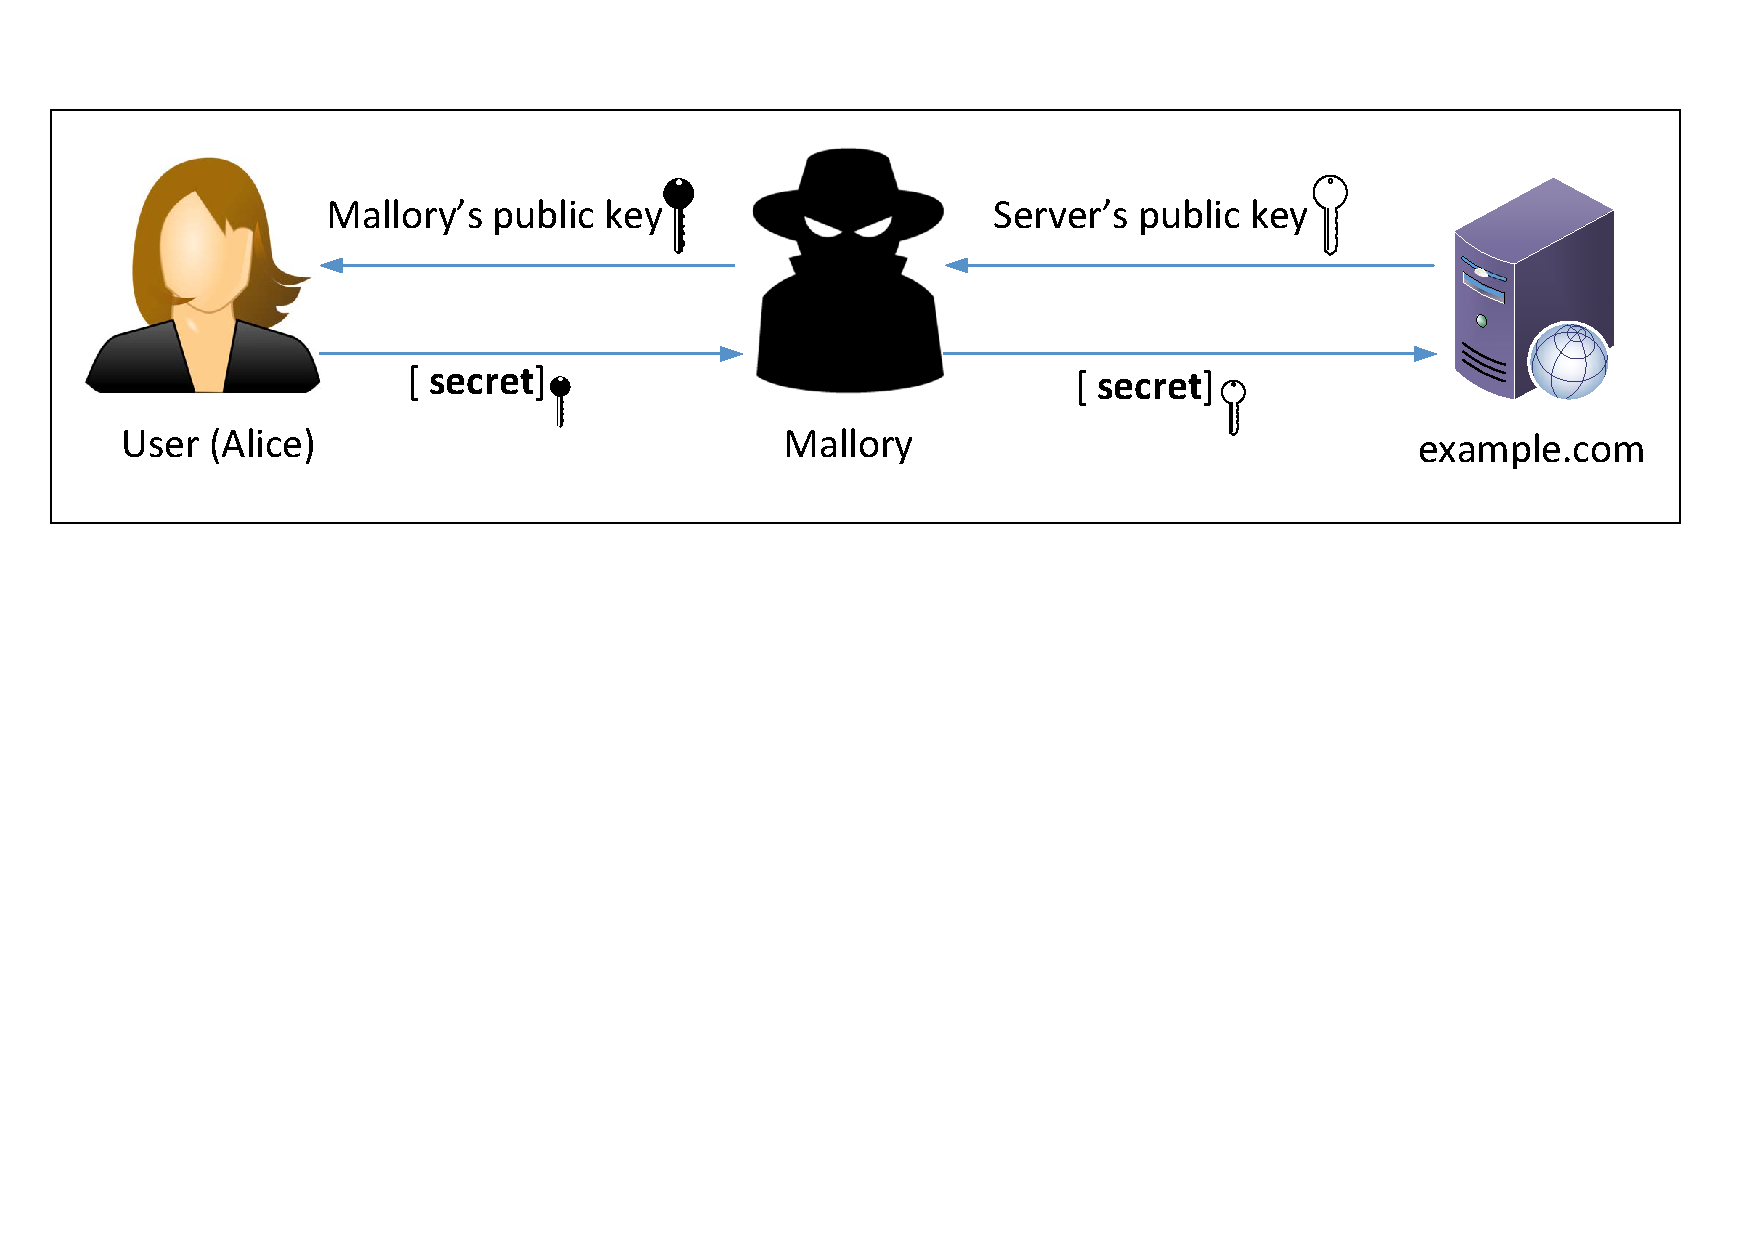
\includegraphics[width=0.8\textwidth]{\pkiFigs/mitm.pdf}
   \end{center}
   \caption{A Man-In-The-Middle (MITM) attack}
   \label{pki:fig:mitm}
\end{figure}



The goal of this task is to help students understand how PKI can defeat such MITM attacks. 
In the task, we will emulate an MITM attack, and see how exactly PKI can defeat it.
We will select a target website first. In this document, we use 
\texttt{example.com} as the target website, but in the task, to make it more meaningful,
students should pick a popular website, such as a banking site and social network site. 


\paragraph{Step 1: Setting up the malicious website.} 
In Task 4, we have already set up an HTTPS website for \pkiserver. We will
use the same Apache server to impersonate \texttt{example.com} (or the site chosen by students).  
To achieve that, we will follow the instruction in Task 4 to 
add a \texttt{VirtualHost} entry to Apache's SSL configuration file: the
\texttt{ServerName} should be \texttt{example.com}, but the rest of the
configuration can be the same as that used in Task 4.
Our goal is the following: when a user tries to visit \texttt{example.com}, 
we are going to get the user to land in our server, which hosts 
a fake website for \texttt{example.com}. If this were a social network
website, The fake site can display a login page similar to the
one in the target website. If users cannot tell the difference, they may type their account credentials
in the fake webpage, essentially disclosing the credentials to the attacker. 


\paragraph{Step 2: Becoming the man in the middle} 
There are several ways to get the user's HTTPS request to land in our web server. One way is to
attack the routing, so the user's HTTPS request is routed to our web server. Another way is
to attack DNS, so when the victim's machine tries to find out the IP address of the target
web server, it gets the IP address of our web server. In this task, we use ``attack'' DNS. Instead of
launching an actual DNS cache poisoning attack, we simply modify the victim's machine's 
\texttt{/etc/hosts} file to emulate the result of a DNS cache positing attack (the
\texttt{IP\_Address} in the following should be replaced by the actual 
IP address of the malicious server).

\begin{lstlisting}[backgroundcolor=]
   <IP_Address>  example.com
\end{lstlisting}


\paragraph{Step 3: Browse the target website.}
With everything set up, now visit the target real website, and 
see what your browser would say. Please explain what you have observed. 




% -------------------------------------------
% SUBSECTION
% ------------------------------------------- 
\subsection{Task 6: Launching a Man-In-The-Middle Attack with a Compromised CA}

Unfortunately, the root CA that we created in Task 1 is compromised by an attacker, and its private
key is stolen. Therefore, the attacker can generate any arbitrary certificate 
using this CA's private key. In this task, we will see 
the consequence of such a compromise. 


Please design an experiment to show that the attacker can successfully launch MITM attacks on
any HTTPS website. You can use the same setting created in Task 5, but this time, you need to
demonstrate that the MITM attack is successful, i.e., the browser will not 
raise any suspicion when the victim tries to visit a website but land in the MITM attacker's
fake website.




% *******************************************
% SECTION
% ******************************************* 
\section{Submission}

\seedsubmission


%%%%%%%%%%%%%%%%%%%%%%%%%%%%%%%%%%%%%%%%%%%%%%%%%%%%%%
\end{document}
%%%%%%%%%%%%%%%%%%%%%%%%%%%%%%%%%%%%%%%%%%%%%%%%%%%%%%

